\documentclass[11pt]{article}
\usepackage[paper=letterpaper,margin=1in]{geometry}
\usepackage[parfill]{parskip}
\usepackage{tikz}
\usetikzlibrary{arrows.meta}
\usepackage{fancyvrb}

\begin{document}
\thispagestyle{empty}

\begin{center}
{\large CS 310}\\
Assignment 408
\end{center}

\begin{flushright}
Brandon Ingli
\end{flushright}

\textbf{Problem 1.} Draw the memo table and memok helper table for the
RNA substructure problem using the RNA sequence CAGUCAUAGCAAUGCU, and
indicate which letters match in the secondary structure.

\textit{Answer:} The memo table appears as 

\begin{center}
\begin{tabular}{ccc|*{12}{c|}}
  \multicolumn{3}{c}{}  & \multicolumn{12}{c}{$j$}  \\
   &    &   & 5 & 6 & 7 & 8 & 9 & 10& 11& 12& 13& 14& 15& 16\\
   &    &   & C & A & U & A & G & C & A & A & U & G & C & U \\\cline{2-15}
   &  0 & --& 0 & 0 & 0 & 0 & 0 & 0 & 0 & 0 & 0 & 0 & 0 & 0 \\\cline{2-15}
   &  1 & C & 0 & 0 & 1 & 1 & 2 & 2 & 2 & 2 & 3 & 4 & 4 & 5 \\\cline{2-15}
   &  2 & A & 0 & 0 & 1 & 1 & 1 & 2 & 2 & 2 & 3 & 3 & 4 & 5 \\\cline{2-15}
   &  3 & G & 0 & 0 & 0 & 0 & 1 & 1 & 2 & 2 & 2 & 3 & 4 & 4 \\\cline{2-15}
   &  4 & U & 0 & 0 & 0 & 1 & 1 & 1 & 2 & 2 & 2 & 3 & 3 & 3 \\\cline{2-15}
   &  5 & C & 0 & 0 & 0 & 0 & 1 & 1 & 1 & 2 & 2 & 3 & 3 & 3 \\\cline{2-15}
$i$&  6 & A &   & 0 & 0 & 0 & 0 & 0 & 0 & 1 & 2 & 2 & 2 & 3 \\\cline{2-15}
   &  7 & U &   &   & 0 & 0 & 0 & 0 & 1 & 1 & 1 & 1 & 2 & 3 \\\cline{2-15}
   &  8 & A &   &   &   & 0 & 0 & 0 & 0 & 0 & 1 & 1 & 2 & 3 \\\cline{2-15}
   &  9 & G &   &   &   &   & 0 & 0 & 0 & 0 & 0 & 0 & 2 & 2 \\\cline{2-15}
   & 10 & C &   &   &   &   &   & 0 & 0 & 0 & 0 & 1 & 1 & 1 \\\cline{2-15}
   & 11 & A &   &   &   &   &   &   & 0 & 0 & 0 & 0 & 0 & 1 \\\cline{2-15}
   & 12 & A &   &   &   &   &   &   &   & 0 & 0 & 0 & 0 & 1 \\\cline{2-15}
\end{tabular}
\end{center}

and the helper memo table appears as
\begin{center}
\begin{tabular}{ccc|*{12}{c|}}
   \multicolumn{3}{c}{}  & \multicolumn{12}{c}{$j$}  \\
   &    &   & 5 & 6 & 7 & 8 & 9 & 10& 11& 12& 13& 14& 15& 16\\
   &    &   & C & A & U & A & G & C & A & A & U & G & C & U \\\cline{2-15}
   &  0 & --&   &   &   &   &   &   &   &   &   &   &   &   \\\cline{2-15}
   &  1 & C &   &   & 2 &   & 1 & 3 & 4 & 4 & 2 & 1 & 3 & 2 \\\cline{2-15}
   &  2 & A &   &   & 2 &   &   & 3 & 4 & 4 & 2 & 5 & 3 & 2 \\\cline{2-15}
   &  3 & G &   &   &   &   &   & 3 & 4 & 4 & 6 & 5 & 3 &   \\\cline{2-15}
   &  4 & U &   &   &   & 4 &   &   & 4 & 4 & 6 & 5 & 9 & 6 \\\cline{2-15}
   &  5 & C &   &   &   &   & 5 &   &   & 7 & 6 & 5 &   & 6 \\\cline{2-15}
$i$&  6 & A &   &   &   &   &   &   &   & 7 & 6 &   & 9 & 6 \\\cline{2-15}
   &  7 & U &   &   &   &   &   &   & 7 & 7 & 8 &   & 9 & 8 \\\cline{2-15}
   &  8 & A &   &   &   &   &   &   &   &   & 8 &   & 9 & 8 \\\cline{2-15}
   &  9 & G &   &   &   &   &   &   &   &   &   &   & 9 &   \\\cline{2-15}
   & 10 & C &   &   &   &   &   &   &   &   &   & 10&   & 11\\\cline{2-15}
   & 11 & A &   &   &   &   &   &   &   &   &   &   &   & 11\\\cline{2-15}
   & 12 & A &   &   &   &   &   &   &   &   &   &   &   & 12\\\cline{2-15}
\end{tabular}
\end{center}

Any values not filled in can be assumed to be 0.

\clearpage

The following letters match up in the RNA Secondary Structure:
\begin{itemize}
   \item (2 - A, 16 - U)
   \item (3 - G, 15 - C)
   \item (5 - C, 14 - G)
   \item (6 - A, 13 - U)
   \item (7 - U, 12 - A)
\end{itemize}

\vspace{22pt}

\textbf{Problem 2.} Given the input 4371, 1323, 6173, 4199, 9679, 1989
for an initially empty hash table, and a hash function 
$h(x) = 6 - (x \bmod 7)$, draw the resulting hash table. State and
explain any assumptions you make, and explain your resulting table.

\textit{Answer:}

\begin{center}
   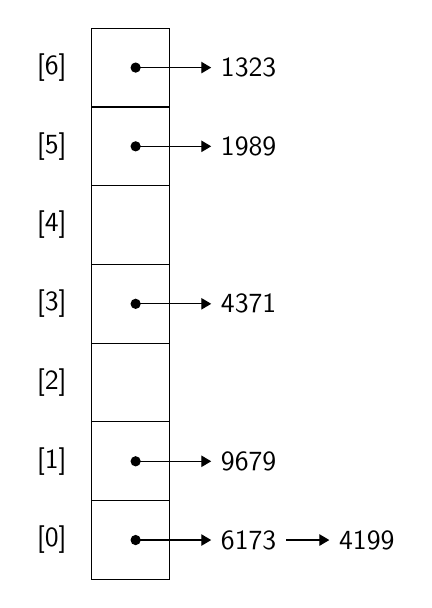
\begin{tikzpicture}[font=\sffamily]
      \draw (1, 6) rectangle (2, 7);
      \draw (1, 5) rectangle (2, 6);
      \draw (1, 4) rectangle (2, 5);
      \draw (1, 3) rectangle (2, 4);
      \draw (1, 2) rectangle (2, 3);
      \draw (1, 1) rectangle (2, 2);
      \draw (1, 0) rectangle (2, 1);
      \node (6) at (0.5, 6.5) {[6]};
      \node (5) at (0.5, 5.5) {[5]};
      \node (4) at (0.5, 4.5) {[4]};
      \node (3) at (0.5, 3.5) {[3]};
      \node (2) at (0.5, 2.5) {[2]};
      \node (1) at (0.5, 1.5) {[1]};
      \node (0) at (0.5, 0.5) {[0]};

      \node (4371) at (3, 3.5) {4371};
      \node (1323) at (3, 6.5) {1323};
      \node (6173) at (3, 0.5) {6173};
      \node (4199) at (4.5, 0.5) {4199};
      \node (9679) at (3, 1.5) {9679};
      \node (1989) at (3, 5.5){1989};

      \draw [Circle-Triangle] (1.5, 0.5) -- (6173);
      \draw [-Triangle] (6173) -- (4199);
      \draw [Circle-Triangle] (1.5, 1.5) -- (9679);
      \draw [Circle-Triangle] (1.5, 3.5) -- (4371);
      \draw [Circle-Triangle] (1.5, 5.5) -- (1989);
      \draw [Circle-Triangle] (1.5, 6.5) -- (1323);

      
   \end{tikzpicture}
\end{center}

From the given hash function, we are assuming a table of size 7, as well as 
open chaining to deal with collisions. The given hash function appears to 
suit the data quite well, as the members are quite evenly distributed. One 
collision occurred at index 0. This table is more than 70\% full.

\clearpage

\textbf{Problem 3.} Rehash the table of problem 2, and show the table that 
results from the rehashing. Explain your process and results.

\textit{Answer:} The next prime number more than twice the size of our 
current table is 17, so that will be the size of our new table. Keeping with 
the spirit of the previous hash function, the new function will be 
$h(x) = 16 - (x \bmod 17)$. After running each element of the previous 
table through the new hash function and placing them in the table, it appears 
as shown below. For the given data, there is one more collision in the rehash 
than in the original table.

\begin{center}
   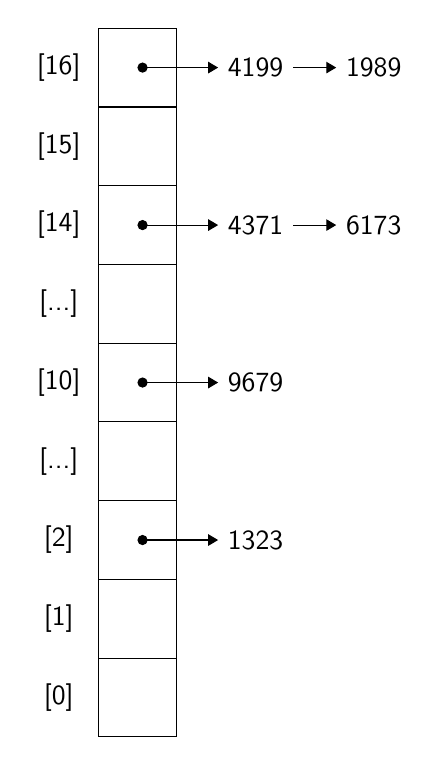
\begin{tikzpicture}[font=\sffamily]
      \draw (1, 8) rectangle (2, 9);
      \draw (1, 7) rectangle (2, 8);
      \draw (1, 6) rectangle (2, 7);
      \draw (1, 5) rectangle (2, 6);
      \draw (1, 4) rectangle (2, 5);
      \draw (1, 3) rectangle (2, 4);
      \draw (1, 2) rectangle (2, 3);
      \draw (1, 1) rectangle (2, 2);
      \draw (1, 0) rectangle (2, 1);
      \node (16) at (0.5, 8.5) {[16]};
      \node (15) at (0.5, 7.5) {[15]};
      \node (14) at (0.5, 6.5) {[14]};
      \node (e2) at (0.5, 5.5) {[...]};
      \node (10) at (0.5, 4.5) {[10]};
      \node (e1) at (0.5, 3.5) {[...]};
      \node (2) at (0.5, 2.5) {[2]};
      \node (1) at (0.5, 1.5) {[1]};
      \node (0) at (0.5, 0.5) {[0]};

      \node (4371) at (3, 6.5) {4371};
      \node (1323) at (3, 2.5) {1323};
      \node (6173) at (4.5, 6.5) {6173};
      \node (4199) at (3, 8.5) {4199};
      \node (9679) at (3, 4.5) {9679};
      \node (1989) at (4.5, 8.5){1989};

      \draw [Circle-Triangle] (1.5, 8.5) -- (4199);
      \draw [-Triangle] (4199) -- (1989);
      \draw [Circle-Triangle] (1.5, 6.5) -- (4371);
      \draw [-Triangle] (4371) -- (6173);
      \draw [Circle-Triangle] (1.5, 4.5) -- (9679);
      \draw [Circle-Triangle] (1.5, 2.5) -- (1323);

   \end{tikzpicture}
\end{center}

\textbf{Problem 4.} Write a program to implement the given hash function and 
count the number of collisions that would occur in a hash table for words 
in the Unix dictionary. Approximate a load factor of 1, and read the words 
from standard input.

\begin{Verbatim}[xleftmargin=5mm]
size_t hash(const string& key, size_t table_size)
{
   size_t hash_val {0};
   for (auto character : key)
   {
      hash_val = 37 * hash_val + static_cast(character);
   }
   return hash_val % table_size;
}
\end{Verbatim}

\textit{Answer:} Please see that attached program. The number of collisions 
detected on my system with 102305 dictionary words was 37633.

\textbf{Problem 5.} Explain and justify your results. Be sure to explain what 
your table size is, and why you chose that value.

\textit{Answer:} To approximate a load factor of 1 with 102305 words, I chose 
a table size of 102301, as this is the closest prime number to the number of 
elements to be placed in the table. About 37\% of the words pushed onto 
the hash table experienced a collision, which can be attributed to the fact 
that the use of letters in the English language is not evenly distributed. 
The data is still somewhat spread out due to the hash function taking the 
length of the word as a major factor in the hash value. While this too is 
not very evenly distributed, the length in combination with letter choice 
helps in spreading the data over the table.
\end{document}
